\chapter{Software Design}

In questo capitolo sono discussi alcuni degli spunti più interessanti e delle soluzioni più ingegnose adottate durante lo sviluppo del software QSapecNG. Viene inoltre illustrata e per quanto possibile descritta nei particolari la procedura generica di ricerca degli alberi di copertura comuni fra due grafi, proposta secondo il modello introdotto da Boost C++ e sottoposta proprio a quest'ultima (all'attenzione della BGL) per l'integrazione.

Per ovvi motivi non è possibile trattare per intero il codice scritto, poiché questo richiederebbe probabilmente svariati capitoli a sé dedicati per essere analizzato nei dettagli e per visitare tutte le relazioni che legano fra loro le diverse parti. Ad ogni modo, nei capitoli che seguiranno sarà discusso l'orientamento adottato durante lo sviluppo, atto a rendere migliorabile e a dare un più ampio respiro al software.


\section{MRT: Tecniche di Programmazione Generica}

Come già anticipato, Boost C++ in primis e quindi la BGL a seguire adottano una metodologia di programmazione generica\graffito{La programmazione generica è uno dei punti cardine del C++ in genere e Boost C++ ne fa uno dei suoi punti di forza, sfruttandone totalmente le potenzialità} con lo scopo di rendere quanto più flessibili tanto le strutture dati quanto gli algoritmi su di esse applicabili. Chi critica Boost C++ prende proprio questo argomento, da cui deriva un aumento di pesantezza in fase di compilazione e un più alto grado di difficoltà d'uso in fase di sviluppo e di partecipazione, come arma per attaccare la libreria. Di contro, però, negli anni la scelta ha ripagato i suoi padri e anche in un modesto lavoro di tesi si è potuto godere dei vantaggi dati, oltre che apportare il proprio contributo.

Allo scopo di aiutare la comprensione di quanto seguirà, è necessario introdurre brevemente alcuni di questi concetti.

\paragraph{Concept} I \textit{concept} rappresentano, detto in parole povere, un meccanismo di controllo sulla conformità di determinati oggetti rispetto a determinati requisiti. Per capirne l'utilità conviene inquadrarli in uno dei loro ambiti d'uso più comune, ovvero i \textit{template}. Quest'ultimi sono sviluppati su un'idea di tipo di dato astratto, sul quale operano, eppure il C++ non fornisce in alcun modo un meccanismo per verificare che il dato sottomesso come parametro sia effettivamente valido (sia cioè un modello per il concetto astratto).\graffito{La peculiarità dei concept è quella di essere composti da codice che in fase di compilazione permette di controllare il rispetto del concetto vero e proprio, mentre all'invocazione del linker viene scartato da quest'ultimo poiché risulta essere non effettivamente utilizzato, pertanto non contribuisce in alcun modo ad appesantire il prodotto finale} Questo può portare a indicazioni hard-coded all'interno dei template stessi o a nomi fantasiosi, che però vengono ignorati dal compilatore (ai fini della compilazione, RandomAccessIterator non è differente da T come nome di parametro). Questo si traduce in:
\begin{itemize}
 \item Errori criptici in fase di compilazione che possono essere forse facilmente decifrabili per un programmatore esperto ma non per chi si è da poco avvicinato al linguaggio.
 \item Mancanza di documentazione o errori sulle specifiche esatte richieste per la conformità di un modello al concetto.
 \item Possibilità che richieste formali in forma di commento risultino difficili da esprimere, con il rischio di diventare troppo blande o più stringenti di quanto non sia realmente necessario.
 \item Concetti documentati nel codice e documentazione per utente finale potrebbero essere discordanti, disorientando quest'ultimo.
\end{itemize}
In questo panorama si collocano pertanto i concept,\graffito{Di fatto i concept forzano una classe ad essere almeno conforme ad una specifica interfaccia, attraverso la quale verrà acceduta} con lo scopo di semplificare la procedura, rendere espliciti i requisiti, rendere maggiormente comprensibili eventuali messaggi di errore e aiutare nel complesso tanto lo sviluppatore quanto l'utente dei template che ne fanno uso (siano essi strutture dati o funzioni generiche, indifferentemente).

\paragraph{Traits} I \textit{traits} rappresentano una delle più importanti tecniche di programmazione generica in C++ e sono ampiamente usati all'interno di Boost C++. Essi permettono di prendere decisioni basate sui tipi in fase di compilazione, così come strutture quali l'\textit{if} permettono di prendere decisioni basate su valori in fase di esecuzione. Per questo motivo i traits vengono spesso chiamati l'\textbf{if-then-else} dei tipi. Essi sono non intrusivi e permettono di associare informazioni ad entità in fase di compilazione.

\paragraph{Tag Dispatching} Questa è una tecnica per sfruttare l'overloading delle funzioni allo scopo di mutarne il comportamento basandosi sulle proprietà di un tipo, letteralmente smistare le richieste fra le diverse funzioni sulla base del tipo fornito come proprietà. Sono spesso usati in concomitanza con l'uso dei traits poiché le proprietà atte allo smistamento sono solitamente accessibili attraverso la tecnica dei traits.

\paragraph{}
Questi sono soltanto alcuni dei principi alla base della programmazione generica, come interpretata in Boost C++. Eppure sono utili poiché rappresentano quei principi la cui comprensione risulterà necessaria per approfondire la discussione dell'algoritmo di ricerca per gli alberi di copertura comuni a due grafi. Ciò nonostante, per chi fosse interessato nei dettagli della singola istruzione, sia chiaro che non è questa la sede per illustrare la logica che sta dietro alle scelte fatte e probabilmente richiederebbe non poco spazio l'affrontare un'analisi dettagliata di un algoritmo, anche semplice, appartenente o proposto per la BGL.

\paragraph{}

\begin{lstlisting}[basicstyle=\small,language=C++,caption={Parte della funzione \textit{mrt}},float,captionpos=b,label={lst:mrtstub},frame=lines,numbers=left]
template <
  class Graph, class Order, class Func, class Seq >
BOOST_CONCEPT_REQUIRES(
  ((RandomAccessContainer<Order>))
  ((IncidenceGraphConcept<Graph>))
  ((UnaryFunction<Func, void, Seq>))
  ((Mutable_RandomAccessContainer<Seq>))
  ((VertexAndEdgeListGraphConcept<Graph>)),
  (void))
mrt_two_graphs_common_spanning_trees
  ( const Graph& iG, Order iG_map,
    const Graph& vG, Order vG_map,
    Func func, Seq inL )
{
  typedef graph_traits<Graph> GraphTraits;

  typedef typename GraphTraits::directed_category directed_category;

  // [...]

  typedef typename GraphTraits::edge_descriptor edge_descriptor;
  typedef typename GraphTraits::edges_size_type edges_size_type;

  // [...]

  typedef typename Seq::value_type seq_value_type;
  typedef typename Seq::size_type seq_size_type;

  // [...]

  typedef typename Order::value_type order_value_type;
  typedef typename Order::size_type order_size_type;

  // [...]

  BOOST_STATIC_ASSERT((is_same<order_value_type, edge_descriptor>::value));
  BOOST_CONCEPT_ASSERT((Convertible<order_size_type, edges_size_type>));
  BOOST_CONCEPT_ASSERT((Convertible<seq_size_type, edges_size_type>));
  BOOST_STATIC_ASSERT((is_same<seq_value_type, bool>::value));
  BOOST_STATIC_ASSERT((is_same<directed_category, undirected_tag>::value));

  // [...]
}
\end{lstlisting}

  Per cominciare, rifacendosi subito ad alcuni dei punti sopra esposti, è molto interessante studiare la parte introduttiva della funzione di ricerca per gli alberi comuni fra due grafi, riportata (opportunamente ripulita dal superfluo per motivi di spazio) nel listato \ref{lst:mrtstub}. Probabilmente all'apparenza piuttosto complessa, tralasciando le dichiarazioni di MACRO prettamente legate a Boost C++, è facilmente interpretabile ed esplicita nelle intenzioni. Inoltre è sufficiente comprendere come essa debba essere invocata, senza dilungarsi sull'effettiva implementazione, per capire un po' meglio l'importanza e l'utilità delle tecniche di sviluppo adottate.\\
  In questo frangente è necessaria una nota: questa non è l'unica chiamata disponibile per la funzione, bensì la più completa. Esistono altre interfacce utilizzabili da chi non voglia sottomettere un ordine (viene usato quello estraibile direttamente dai grafi stessi) o per chi non intenda usufruire degli alberi individuati, sebbene questo abbia di per sé poca utilità ai fini pratici.

\begin{figure}[t]
 \centering
 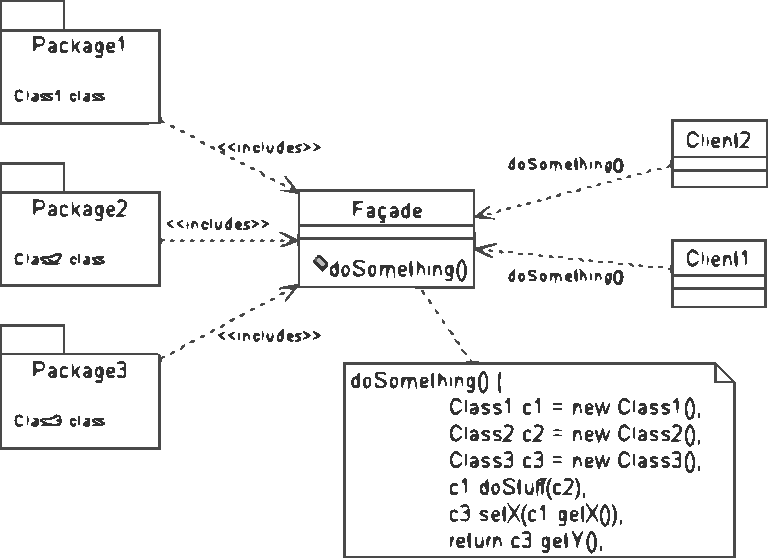
\includegraphics[scale=0.80]{immagini/facade.pdf}
 \caption{Pattern Facade, modello per la funzione \textit{mrt}}
 \label{fig:facade}
\end{figure}

La funzione \textit{mrt} rappresenta il punto di ingresso per un labirinto ben più articolato di strutture dati e chiamate a funzione, celato all'utente finale e accessibile attraverso una semplice chiamata ad essa. Rifacendosi al pattern \textit{Facade},\graffito{Il pattern Facade è molto importante, poiché permette di celare dietro un'amichevole chiamata di funzione la complessità di una serie di operazioni che risulterebbero estremamente complesse nel loro utilizzo se lasciate all'utente} riportato in figura \ref{fig:facade}, questa funzione nasconde al suo interno l'approccio ricorsivo dell'algoritmo e tutte quelle richieste e definizioni di strutture necessarie all'espletamento dei propri compiti.

Come si nota ad una prima occhiata, essa sfrutta le possibilità offerte dalla programmazione generica e richiede di essere parametrizzata su:
\begin{itemize}
 \item Un modello di grafo, \textit{Graph}, a cui i due grafi sottomessi su cui effettuare la ricerca dovranno essere conformi.
 \item Un modello di ordine, \textit{Order}, ovvero una struttura atta all'utilizzo per l'interrogazione relativa all'indice associato ai singoli archi.
 \item Un modello di funzione, \textit{Func}, utilizzata prevalentemente per l'invocazione su ogni albero individuato.
 \item Un modello di contenitore, \textit{Seq}, per immagazzinare gli archi via via che vengono inseriti nei potenziali alberi.
\end{itemize}
Sebbene al momento possano risultare abbastanza oscuri i veri utilizzi di questi oggetti, saranno chiari a breve, ovvero una volta osservati i concetti a cui devono rifarsi. Seguendo lo stesso ordine di cui sopra, studiando meglio il tutto:
\begin{itemize}
 \item Per quanto riguarda Graph, le prime cose da osservare sono due dichiarazioni che ne definiscono completamente la struttura, ovvero:
   \begin{enumerate}
    \item La necessità che esso sia conforme al concetto (definito dalla BGL stessa) di \textit{IncidenceGraph} (riga 5), un'interfaccia che permette un accesso efficiente per gli archi in uscita dal singolo vertice.
    \item La necessità che esso sia conforme al concetto (definito dalla BGL stessa) di \textit{VertexAndEdgeListGraph} (riga 8), il quale permette l'attraversamento di tutti i vertici e l'accesso a tutti gli archi in modo semplice ed immediato.
   \end{enumerate}
 Queste richieste sono legate anche e non solo agli algoritmi base utilizzati, già presenti nella BGL e quindi non re-implementati, e ai loro vincoli di concetto. Meno interessanti le definizioni che seguono, molte delle quali saranno discusse anche nei punti seguenti poiché relative pure ad altri elementi. Da sottolineare la presenza (riga 40) dell'imposizione sul fatto che il grafo sia non orientato: questo è necessario per i motivi già esposti nei capitoli precedenti, poiché permette un corretto accesso al grafo e non esclude il fatto che si possa conoscere l'effettivo orientamento del singolo arco attraverso la sua definizione, che porta con sé intrinsecamente tale informazione. Ancora, da notare come quest'ultimo particolare sia alla base del \textit{tag dispatching}.
 \item La prima dichiarazione pilota il modello Order (riga 4), affermando che esso deve essere conforme a quello di un contenitore ad accesso causale, come definito in \cite{STL}. Banalmente questo dovrebbe far subito intuire che la volontà è quella di rendere Order un contenitore di tipo vettore a cui si accede tramite la definizione di un arco, ottenendone l'indice associato (o meglio, accedendo con l'$i_{esimo}$ indice si ricava l'arco associato, che rappresenta poi in realtà la soluzione effettivamente adottata in QSapecNG nella forma di un vettore). Proseguendo infatti nello studio delle definizioni associate ad Order si ha che, a seguito di una ridenominazione delle informazioni contenute (righe 31-32, per semplicità d'uso), viene accertata l'equivalenza fra il tipo dati contenuti e quello che descrive effettivamente un arco e quindi verificata la convertibilità fra le tipologie di indicizzazione nei due spazi (righe 36-37).
 \item Come detto parlando a proposito di Func, questo oggetto rappresenta il prototipo di una funzione a cui verranno sottomessi gli alberi di copertura comuni, una volta individuati. Poiché Seq è destinato a contenere gli archi di tali alberi prima, durante e a costruzione finita, Func riceverà in ingresso proprio tale lista (riga 6) restituendo niente in uscita. Questo è, di fatto, sufficiente a descrivere completamente l'oggetto Func, delegando agli altri elementi tutto il resto (tipo di archi, di indici, etc.).
 \item Ultimo ma non meno importante è Seq, che rappresenta un contenitore per mantenere gli archi dell'albero di copertura comune ai due grafi durante la ricerca (ovvero, la costruzione). In particolare (riga 7) viene richiesto che, come già successo per Order, esso sia definito come un contenitore ad accesso causale ma con la particolarità di essere modificabile (intuitivamente è destinato ad un uso di inserimento e rimozione di elementi al suo interno o di modifica di quest'ultimi). Procedendo, però, si ricavano informazioni in grado di chiarire il vero scopo di Seq (righe 38-39). Viene infatti verificata la convertibilità dei suoi indici di accesso con quelli che permettono di accedere agli archi all'interno di un grafo, ma ancora più importante viene imposto che il tipo di dato contenuto sia una variabile booleana. Se fosse stato riportato uno spezzone maggiore di software, si sarebbe potuto notare anche la verifica in codice sulla stessa dimensione dei due spazi (ovvero sul fatto che i componenti contenuti in Seq fossero in numero pari agli archi da analizzare). Riassumendo: a partire dagli elementi ottenuti, quindi, si deduce che Seq potrà essere ad esempio rappresentato da un vettore di dimensione pari al numero di archi nei due grafi e contenente variabili booleane, le quali indicano la presenza (\textbf{true}) o meno (\textbf{false}) dell'$i_{esimo}$ arco all'interno del $j_{esimo}$ albero.
\end{itemize}

Con queste poche nozioni si riesce a modellare in maniera sufficientemente facile un ambiente in grado di istanziare, inizializzare e sottomettere i corretti oggetti alla funzione di ricerca per gli alberi comuni fra due grafi. Il resto del codice si riduce a mere chiamate alle funzioni fornite dalla BGL che ricalcano fedelmente l'algoritmo esposto nei capitoli precedenti e non è pertanto di pari interesse.

\paragraph{}

\begin{lstlisting}[basicstyle=\small,language=C++,caption={Tree Collector},float,captionpos=b,label={lst:treecoll},frame=lines,numbers=left]
template <class Coll, class Seq>
struct tree_collector
{

public:
  BOOST_CONCEPT_ASSERT((BackInsertionSequence<Coll>));
  BOOST_CONCEPT_ASSERT((RandomAccessContainer<Seq>));
  BOOST_CONCEPT_ASSERT((CopyConstructible<Seq>));

  typedef typename Coll::value_type coll_value_type;
  typedef typename Seq::value_type seq_value_type;

  BOOST_STATIC_ASSERT((is_same<coll_value_type, Seq>::value));
  BOOST_STATIC_ASSERT((is_same<seq_value_type, bool>::value));

  tree_collector(Coll& seqs): seqs_(seqs) { }

  inline void operator()(Seq seq)
    { seqs_.push_back(seq); }

private:
  Coll& seqs_;

};
\end{lstlisting}

Un ultimo aspetto, sempre legato ai concetti della programmazione generica, è rappresentato dall'oggetto fornito a supporto per l'uso con la funzione \textit{mrt}, riportato per intero nel listato \ref{lst:treecoll}. I due elementi che riceve come argomento in questo caso dovranno rispettare i seguenti vincoli:
\begin{itemize}
 \item Per quanto riguarda \textit{Coll}, si richiede che esso permetta un inserimento in coda (ne sono modelli vettori, liste, etc.).
 \item Per quanto riguarda invece Seq, viene richiesta la possibilità di accesso casuale (già discussa) e la possibilità di copia. Se si pensa alla necessità di immagazzinare gli alberi di volta in volta proposti come validi, si intuisce immediatamente il perché di quest'ultima domanda.
\end{itemize}
Per entrambi poi vi sono vincoli che li legano all'altro, ovvero innanzitutto si verifica che il tipo ospitato da Coll sia proprio Seq (qui diventa chiaro che Coll è un deposito destinato ad ospitare i diversi alberi, i quali anche se non esplicitamente dichiarato saranno con molta probabilità definiti da Seq), quindi viene forzato il tipo di Seq ad una variabile booleana. Questo aspetto è molto importante perché si rifà anche ai vincoli imposti dalla funzione analizzata in precedenza; infatti, se guardiamo al \textit{Tree Collector} come ad un oggetto funzione (per come è definito, lo è a tutti gli effetti) che sia accettato dalla procedura di ricerca \textit{mrt} (ancora una affermazione vera, basta osservare la dichiarazione stessa dell'operatore), allora segue che il tipo da esso accettato deve ricalcare il tipo che a priori sappiamo gli sarà proposto dalla procedura stessa.

\paragraph{}
Quanto brevemente accennato in questa sezione sono alcuni dei rudimenti della programmazione generica, abbracciata e ampiamente utilizzata nello sviluppo di QSapecNG. Per chi fosse interessato ai dettagli si rimanda al codice del software e alla letteratura in merito.

\section{Qt e il modello signal/slot}

\begin{figure}[ht]
 \centering
 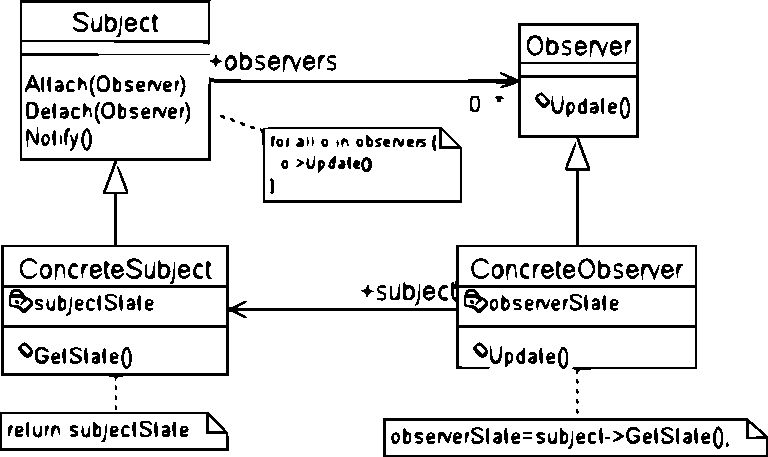
\includegraphics[scale=0.80]{immagini/observer.pdf}
 \caption{Pattern Observer}
 \label{fig:observer}
\end{figure}

Nella panoramica sui risvolti più interessanti del codice è necessario citare il modello \textbf{signal-slot} offerto dalle librerie Qt, sebbene questo non sia stato propriamente applicato quanto piacevolmente adottato per migliorare il software e rendere più flessibile la programmazione. In parole povere, questo modello si propone come un'ottima alternativa al sistema delle callback, mimando il pattern \textit{Observer} (si veda figura \ref{fig:observer}) e al contempo liberando l'utente dalla scrittura del codice di controllo ridondante e sempre uguale che vi fa da contorno.

Gli attori sono banalmente presentati e descritti come:
\begin{description}
 \item[signal] Sono emessi da un oggetto quando muta il proprio stato interno in un modo che può essere interessante per chi lo possiede o per chi lo osserva. Intuitivamente solo chi definisce il segnale e le sottoclassi possono emettere la notifica di cambiamento. Quando un segnale viene emesso, tutti gli slot ad esso collegati vengono invocati in successione, indipendentemente dal ciclo di esecuzione principale (ad esempio, in caso di interfacce grafiche).
 \item[slot] Uno slot rappresenta un metodo avente firma identica in tutto e per tutto ai segnali al quale lo si vuole collegare, che viene invocato quando tali segnali sono emessi. In quanto funzione, esso può essere chiamato anche direttamente da altre classi, se pubblico, o da classi ereditarie.
\end{description}

Alcune particolarità che distinguono la coppia \textit{signal-slot} dagli altri metodi sono:
\begin{itemize}
 \item L'essere un metodo type-safe: le firme di signal e slot devono coincidere e non vi è la possibilità di confusione o errori sul passaggio di valori.
 \item La capacità di abbattere l'accoppiamento fra le classi, riducendolo al minimo indispensabile per permettere la comunicazione fra esse. Di fatto chi emette un segnale non si preoccupa minimamente di chi siano i riceventi.
 \item Arbitrarietà sul numero e sul tipo di componenti passate come argomento alla chiamata.
 \item Possibilità di connettere più segnali ad un unico slot, più slot ad un unico segnale e perfino più segnali in cascata fra loro.
\end{itemize}
Tutto sommato, insomma, il meccanismo in questione rappresenta una utile e potente tecnica di programmazione capace di semplificare non poco le cose.

Ovviamente la questione è sufficientemente più articolata e complessa; si possono per esempio definire slot virtuali e realizzare cose ben più raffinate. Ad ogni modo non è questa la sede per discutere di un metodo dovuto e legato ad una libreria semplicemente sfruttata durante lo sviluppo di QSapecNG, poiché la documentazione che accompagna tale libreria risulta essere più che esaustiva in merito.

\section{Design Patterns}
A conclusione di questa panoramica sulle tecniche di sviluppo adottate, vengono descritti alcuni degli approcci utilizzati per risolvere problemi tipici della programmazione ad oggetti, riscontrabili anche nel software in esame. Queste tecniche prendono il nome di \textit{Design Pattern} (schema di progettazione) e rappresentano soluzioni generali a problemi ricorrenti nella programmazione. I design pattern non sono oggetti o librerie pronte all'uso quanto piuttosto modelli da applicare in frangenti noti, riuscendo a risolvere così in modo elegante, pulito e maggiormente manutenibile le problematiche reali.

\paragraph{Pattern Monostate}

\begin{lstlisting}[basicstyle=\small,language=C++,caption={Pattern Singleton},float,label={lst:singleton},captionpos=b,frame=lines]
 class Singleton
 {
 private:
   static Singleton* instance;

   Singleton(): some_data(0) { }
   ~Singleton() { }
   Singleton(const Singleton &);
   Singleton & operator=(const Singleton &);

   int some_data;

 public:
   static Singleton& get_instance();

   void increment() { ++some_data; }
   int get_data() { return some_data; }
 };


 Singleton Singleton::instance = 0;


 Singleton& Singleton::get_instance()
 {
   if(!instance)
     instance = new Singleton;

   return *instance;
 }
\end{lstlisting}

\begin{lstlisting}[basicstyle=\small,language=C++,caption={Pattern Monostate},float,label={lst:monostate},captionpos=b,frame=lines]
 class Monostate
 {
 private:
   static int some_data;

 public:
   Monostate() { }
   ~Monostate() { } 

   void increment() { ++Monostate::some_data; }
   int get_data() { return Monostate::some_data; }
 };


 int Monostate::some_data = 0;
\end{lstlisting}

\begin{lstlisting}[basicstyle=\small,language=C++,caption={Pattern Monostate in QSapecNG},float,label={lst:qmono},captionpos=b,frame=lines]
class SettingsManager;


class Settings
{

friend class SettingsManager;

public:
  Settings() { }

  inline int logLvl() const
    { return logLvl_; }

  inline QColor debugColor() const
    { return debugColor_; }

  inline QColor infoColor() const
    { return infoColor_; }

  // ...

private:
  static int logLvl_;
  static QColor debugColor_;
  static QColor infoColor_;

  // ...

};

int Settings::logLvl_ = 0;
QColor Settings::debugColor_ = QColor(Qt::black);
QColor Settings::infoColor_ = QColor(Qt::black);

// ...


class SettingsManager
{

public:
  inline void setLogLvl(int lvl)
    { Settings::logLvl_= lvl; }

  inline void setDebugColor(const QColor& color)
    { Settings::debugColor_ = color; }

  inline void setInfoColor(const QColor& color)
    { Settings::infoColor_ = color; }

  // ...

};
\end{lstlisting}

Uno dei pattern più discussi e criticati è il \textit{Singleton} (listato \ref{lst:singleton}), un approccio atto a rendere centralizzata in un singolo oggetto la possibilità di istanziare una classe e disporne riferimenti per l'accesso ai dati. Risulta utile quando è necessario che sia un solo oggetto a gestire l'accesso a determinate funzioni e parametri all'interno dell'intero ambiente. Il rovescio della medaglia è dato dal fatto che l'uso di questo pattern rende difficoltose le fasi di testing del software ed introduce uno stato globale nell'applicazione. Riduce inoltre le potenzialità del parallelismo, obbligando la serializzazione in accesso e qualcuno lo annota addirittura fra gli \textit{anti-pattern}, ovvero tutte quelle tecniche che rappresentano un modo sbagliato di procedere nella programmazione.\\
Il problema fondamentale del pattern Singleton è che esso rende unico l'oggetto istanziabile e utilizzabile per l'accesso ai dati, rappresentando una sorta di collo di bottiglia per l'uso di informazioni che sarebbero altrimenti rese a livello globale. Se si permettesse, infatti, la creazione di più oggetti Singleton, ognuno di essi conterrebbe informazioni che finirebbero con l'essere discordanti nel tempo, rendendo di fatto incoerente lo stato globale all'interno del sistema. In altri termini, istanziando più oggetti Singleton, ogni loro utilizzatore avrebbe un'immagine diversa del sistema, in base all'oggetto a cui accede.

Come alternativa al pattern Singleton, è stato proposto negli anni il pattern \textit{Monostate}\graffito{Il pattern Monostate espone gli stessi punti deboli del pattern Singleton ma è maggiormente apprezzato perché favorisce soluzioni più pulite ai problemi intrinseci} (listato \ref{lst:monostate}). Questo è definito a livello concettuale come un Singleton ma sfrutta la possibilità di rovesciare il punto di vista. Non è più l'oggetto che gestisce i dati ad essere unico nel sistema, bensì sono i dati ad essere unici, ovvero statici e privati. Questo non risolve, in realtà, tutte le problematiche legate al pattern Singleton, sebbene ne renda più snello e chiaro l'uso. Un oggetto Monostate si presta meglio anche all'uso in ambienti paralleli, poiché la serializzazione non avviene più all'esterno ma può essere spostata all'interno dell'oggetto. Inoltre viene meno la necessità di avere un unico oggetto istanziato all'interno del sistema e se ne possono avere in numero illimitato.

All'interno di QSapecNG il pattern Monostate è stato utilizzato principalmente per centralizzare la gestione dei dati di configurazione dell'interfaccia grafica, così da permetterne un facile accesso da qualsiasi punto. Il modello adottato è leggermente diverso da quello visto nel listato \ref{lst:monostate} ed è parzialmente riportato nel listato \ref{lst:qmono}, dove si nota come siano suddivise fra loro la classe utilizzata per l'accesso in lettura e la memorizzazione dei dati e quella indicata per l'accesso in scrittura.

\paragraph{Pattern Builder}

\begin{figure}[ht]
 \centering
 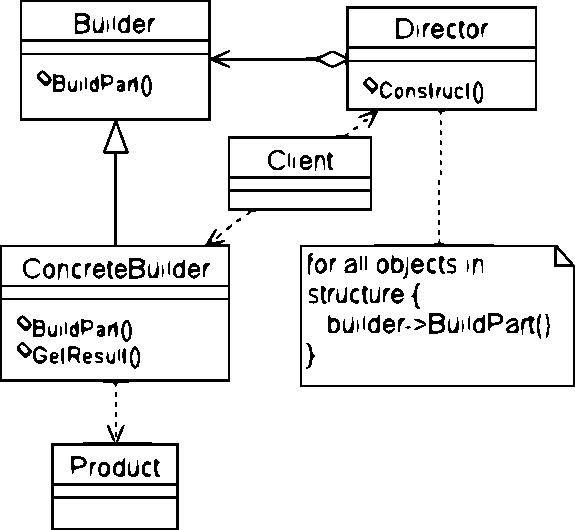
\includegraphics[scale=0.80]{immagini/builder.pdf}
 \caption{Pattern Builder}
 \label{fig:builder}
\end{figure}

Il pattern \textit{Builder} (riportato in figura \ref{fig:builder}) si è rivelato il più flessibile e meglio integrato nell'intera struttura del software QSapecNG. Gli intenti alla base di questo modello sono i seguenti:
\begin{itemize}
 \item Separare le procedure di costruzione di un oggetto complesso dalla sua rappresentazione.
 \item Fare in modo che uno stesso processo di generazione possa dar luogo a più rappresentazioni diverse.
\end{itemize}
Questo lo si ottiene a partire da due classi, chiamate spesso in letteratura \textit{Director} e \textit{Builder}, di cui la seconda è una semplice interfaccia. Le rappresentazioni concrete di Builder andranno quindi a costituire il processo di generazione dei diversi oggetti, mentre a Director sarà demandato il compito di orchestrare correttamente la chiamata dei singoli metodi. Infine, le classi che ereditano da Builder potranno fornire metodi ausiliari per recuperare quanto creato al loro interno.

\begin{lstlisting}[basicstyle=\small,language=C++,caption={Builder in QSapecNG},float,label={lst:builder},captionpos=b,frame=lines]
class abstract_builder
{

public:
  enum const_vertex { GROUND = 0 };

  enum dual_component_type
    { R, G, L, C, V, I, VM, AM };

  enum quad_component_type
    { VCCS, VCVS, CCCS, CCVS, AO, n, K };

public:
  virtual ~abstract_builder() { }

  virtual void add_circuit_properties(
    std::map<std::string, std::string> map) = 0;
  virtual void add_circuit_property(
    std::string name, std::string value) = 0;

  virtual void add_wire_component(
      std::map<std::string, std::string> props =
        std::map<std::string, std::string>()
    ) = 0;

  virtual void add_out_component(
      unsigned int v,
      std::map<std::string, std::string> props =
        std::map<std::string, std::string>()
    ) = 0;

  virtual void add_dual_component(
      dual_component_type c_type,
      std::string name, double value, bool symbolic,
      unsigned int va, unsigned int vb,
      std::map<std::string, std::string> props =
        std::map<std::string, std::string>()
    ) = 0;

  virtual void add_quad_component(
      quad_component_type c_type,
      std::string name, double value, bool symbolic,
      unsigned int va, unsigned int vb,
      unsigned int vac, unsigned int vbc,
      std::map<std::string, std::string> props =
        std::map<std::string, std::string>()
    ) = 0;

  virtual void add_unknow_component(
      std::map<std::string, std::string> props =
        std::map<std::string, std::string>()
    ) = 0;

  virtual void flush() = 0;

};
\end{lstlisting}

\begin{lstlisting}[basicstyle=\small,language=C++,caption={Director in QSapecNG},float,label={lst:parser},captionpos=b,frame=lines]
class abstract_parser
{

public:
  abstract_parser() { }
  virtual ~abstract_parser() { }

  virtual void parse(abstract_builder& builder) = 0;

};
\end{lstlisting}

Astraendo ulteriormente si può pensare di rendere anche la classe Director una semplice interfaccia, costruendo un doppio albero di ereditarietà che permetta la costruzione di oggetti diversi a partire da sorgenti diverse. Questo è stato l'approccio utilizzato in QSapecNG e le interfacce base sono riportate integralmente nei listati \ref{lst:builder} e \ref{lst:parser}.

Le potenzialità di questo approccio sono state sfruttate in diversi punti del software. I più rilevanti sono:
\begin{itemize}
 \item Una classe ereditata da Builder capace di costruire circuiti schematici in base alle sollecitazioni.
 \item Una classe ereditata da Parser capace di leggere ed interpretare circuiti schematici.
 \item Una classe ereditata da Builder per la generazione del circuito come coppia di grafi in corrente e in tensione.
 \item Più classi ideate con lo scopo di leggere e scrivere file su disco, per la memorizzazione ed il caricamento di dati.
\end{itemize}
Questi sono solamente alcuni dei casi in cui è stato applicato il pattern in questione ma se ne intuisce facilmente l'utilità.\\
Immaginiamo per esempio di voler generare, a partire da un disegno schematico, una coppia di grafi in corrente e in tensione: basterà agganciare l'apposito Builder al Director in grado di leggere lo schema. Non solo, volendo si può anche by-passare il disegno dello schema e perfino l'avvio dell'interfaccia grafica, utilizzando un Parser per la lettura di file da disco unito al Builder di cui sopra. Se poi il disegno dello schema lo si vuole evitare perché, semplicemente, lo si è già disegnato, all'ultimo Parser utilizzato basterà legare un Builder capace di generare il circuito schematico ed il gioco è fatto.\\
Questa tecnica può anche essere utilizzata in frangenti meno ovvi, ad esempio nelle fasi di copia-incolla, leggendo da uno schema circuitale su di uno flusso di testo e quindi, attingendo da quest'ultimo, sfruttando un costruttore per incollare quanto copiato.

Riassumendo quindi si nota come il pattern Builder si presti a realizzare una gran quantità di interconnessioni fra oggetti anche in aree diverse del software, disaccoppiando o rendendo comunque minimo l'accoppiamento fra essi e permettendo di risolvere elegantemente problemi che avrebbero altrimenti richiesto la stesura di classi dalla collocazione dubbia, ambigue nel comportamento e difficilmente manutenibili.

\paragraph{Pattern Template Method}

\begin{figure}[ht]
 \centering
 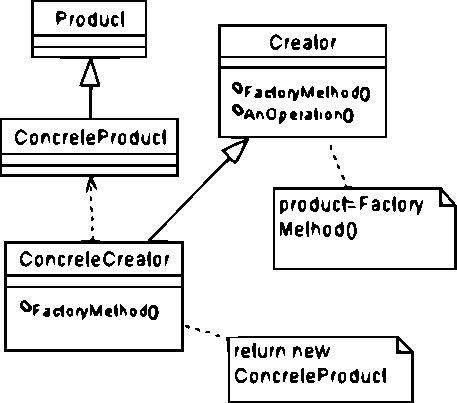
\includegraphics{immagini/factorymethod.pdf}
 \caption{Pattern Factory Method}
 \label{fig:factorymethod}
\end{figure}

\begin{lstlisting}[basicstyle=\small,language=C++,caption={Pattern Template Method in QSapecNG},float,label={lst:templatemethod},captionpos=b,frame=lines]
struct functor
{

public:
  std::pair< std::vector<double>, std::vector<double> >
  operator()
    (
      const metacircuit::expression& numerator,
      const metacircuit::expression& denominator,
      std::map< std::string, double > values
    )
  {
    std::map< int, double > real_num = synthesis(numerator, values);
    std::map< int, double > real_den = synthesis(denominator, values);
    return op(real_num, real_den);
  }

protected:
  virtual std::pair< std::vector<double>, std::vector<double> >
    op(std::map< int, double > num, std::map< int, double > den) = 0;

private:
  std::map< int, double >
  synthesis(
      const metacircuit::expression& expr,
      std::map< std::string, double > values
    )
  {
    // ...
  }

};
\end{lstlisting}

Questo pattern (illustrato in figura \ref{fig:factorymethod}) è particolarmente interessante poiché sfrutta i principi della \textit{IoC} (\textit{Inversion of Control}, o inversione di controllo), ovvero ribalta il meccanismo dell'ereditarietà. Non sono più infatti le classi che ereditano a chiamare i metodi della classe base, bensì sarà quest'ultima ad invocare uno o più metodi lasciati da implementare alle classi derivate. Si riesce così a definire la struttura di un algoritmo delegando alle sottoclassi il compito di implementare i passi chiave, permettendone una personalizzazione ma evitando al contempo la duplicazione di codice. Questo modus operandi (largamente usato anche in diversi framework noti) è detto \textit{Principio di Hollywood: ``non chiamarci, ti chiameremo noi''}.

All'interno del codice di QSapecNG questo modello è stato adottato per le diverse funzioni applicabili ad un determinato circuito, in modo da costruire un'architettura robusta ma personalizzabile per l'analisi dei dati derivati dalla simulazione. Nel listato \ref{lst:templatemethod} è riportata la classe base (classe funzione, per inciso), dove si nota la chiamata del metodo la cui implementazione è lasciata come onere alle classi derivate.

Per completezza di informazione bisogna dire che da questa classe base ereditano classi come ad esempio \textit{gain} o \textit{zeros} e così via, il cui nome è esplicativo della funzione svolta. Salendo di livello e spostandoci da SapecNG, dove tale modello è sviluppato, a QSapecNG, dove tale modello è effettivamente sfruttato, si può osservare come queste classi derivate si vadano a collocare in un'architettura di \textit{traits} che ne completa l'informazione associata, arricchendola nell'ottica dell'uso all'interno dell'interfaccia grafica. Questo lascia intuire come le varie parti del sistema e i diversi pattern possano venire in contatto e collaborare fra loro per uno scopo comune.
